\documentclass[aspectratio=169, 11pt]{beamer}

\usetheme{Madrid}
\usecolortheme{whale}
\setbeamertemplate{navigation symbols}{}
\setcounter{tocdepth}{1}
\AtBeginSection{\begin{frame}\centering{\usebeamercolor[fg]{structure}\Huge\bfseries\insertsection}\end{frame}}

% Custom colors
\definecolor{tuwblue}{RGB}{0,102,153}
\definecolor{tuwgray}{RGB}{128,128,128}
\definecolor{successgreen}{RGB}{34,139,34}
\definecolor{failred}{RGB}{178,34,34}

% Custom colors
\definecolor{tuwblue}{RGB}{0,102,153}
\definecolor{tuwgray}{RGB}{128,128,128}
\definecolor{successgreen}{RGB}{34,139,34}
\definecolor{failred}{RGB}{178,34,34}

\setbeamercolor{title}{fg=white,bg=tuwblue}
\setbeamercolor{frametitle}{fg=white}
\setbeamercolor{structure}{fg=tuwblue}

\usepackage[utf8]{inputenc}
\usepackage[T1]{fontenc}
\usepackage{hyperref}
\usepackage{booktabs}
\usepackage{amsfonts}
\usepackage{amsmath}
\usepackage{graphicx}
\usepackage{xcolor}

\title[PPO on CartPole]{Reinforcement Learning: PPO on CartPole}
\subtitle{Introduction to Deep Learning}

\author{%
  Lukas Leeb \and
  Michael Gail
}

\institute[TU Wien]{Technical University of Vienna}

\date{\today}

\begin{document}

\begin{frame}
  \titlepage
\end{frame}

\begin{frame}{Outline}
  \tableofcontents
\end{frame}

\section{Introduction and Terms}

\subsection{Reinforcement Learning Definition}
\begin{frame}{Reinforcement Learning Definition}
  \centering
  This slide will introduce the formal definition of reinforcement learning and the agent-environment interaction loop.
\end{frame}

\subsection{Reinforcement Learning Environment}
\begin{frame}{Reinforcement Learning Environment}
  \centering
  This slide will describe how an RL environment is modeled as a Markov Decision Process (MDP) (within gymnasium).
\end{frame}

\subsection{CartPole Environment}
\begin{frame}{CartPole Environment\footnote[frame]{Gymnasium: \url{https://gymnasium.farama.org/environments/classic_control/cart_pole/}}}
  \begin{columns}
    \begin{column}{0.35\textwidth}
      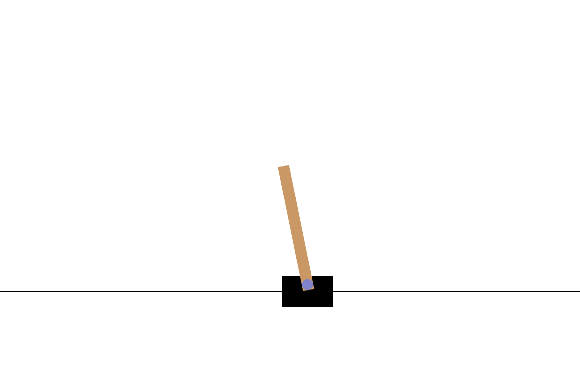
\includegraphics[width=\textwidth]{assets/CartPole.png}
    \end{column}
    \begin{column}{0.65\textwidth}
      A pole is attached to a cart moving along a frictionless track.
      \vfill
      \textbf{Goal:} Keep the pole balanced by applying left or right
      forces.
      \vfill
      \textbf{Action space:} $0$ (left), $1$ (right)
      \vfill
      \textbf{Observation space:}
      \begin{itemize}
        \item Cart position $\in [-4.8, 4.8]$
        \item Cart velocity $\in (-\infty, \infty)$
        \item Pole angle $\in [-24^\circ, 24^\circ]$
        \item Pole angular velocity $\in (-\infty, \infty)$
      \end{itemize}
      \vfill
      \textbf{Reward:} $1$ per step while not terminated
      \vfill
      \textbf{Termination:}
      \begin{itemize}
        \item Pole angle exceeds $\pm 12^\circ$
        \item Cart leaves area $[-2.4,2.4]$
      \end{itemize}
    \end{column}
  \end{columns}
\end{frame}

\subsection{Reinforcement Learning and PPO}
\begin{frame}{Reinforcement Learning and PPO}
  \centering
  This slide will explain where in the Reinforcement Learning Process PPO fits in.
\end{frame}

\section{Proximal Policy Optimization}

\subsection{How PPO Works}
\begin{frame}{How PPO Works}
  \centering
  This slide will provide a high-level overview of the PPO algorithm.
\end{frame}

\subsection{Mathematical Formulation}
\begin{frame}{Mathematical Formulation}
  \centering
  This slide will present the core PPO loss function, ...
\end{frame}

\subsection{Algorithm Pseudocode}
\begin{frame}{Algorithm Pseudocode}
  \centering
  This slide will show the pseudocode for the PPO training loop with rollout collection and mini-batch updates.
\end{frame}

\section{Experiment Setup}

\subsection{Network Architecture}
\begin{frame}{Network Architecture}
  \centering
  This slide will describe the actor and critic network architectures used in our implementation.
\end{frame}

\subsection{Hyperparameters}
\begin{frame}{Hyperparameters}
  \centering
  This slide will list the hyperparameters used for training, including learning rate, clipping parameter, GAE lambda, and rollout length.
\end{frame}

\subsection{Evaluation Metrics}
\begin{frame}{Evaluation Metrics}
  \centering
  This slide will define the metrics used to evaluate performance, such as average episode return and stability across seeds.
\end{frame}

\section{Results}

\begin{frame}{Results}
  \centering
  This slide will present the training curves and final performance of PPO on CartPole.
\end{frame}

\end{document}
